\section{Sensor de temperatura}

El sensor de temperatura MAX30205 tiene una interfaz de comunicación I2C, para poder comprobar su funcionamiento de forma unitaria, fue necesario configurar la interfaz I2C con la que cuenta el dsPIC30205 y adicionalmente crear las rutinas para mantener la comunicación entre ambos componentes.\\

En la figura \ref{fig:DiagramaMAX30205} se muestra en diagrama de tiempo que describe el procedimiento que debe ser seguido para realizar la comunicación entre el MAX30205 y el dsPIC.\\


\begin{figure}[htbp!]
	\centering
	\fbox{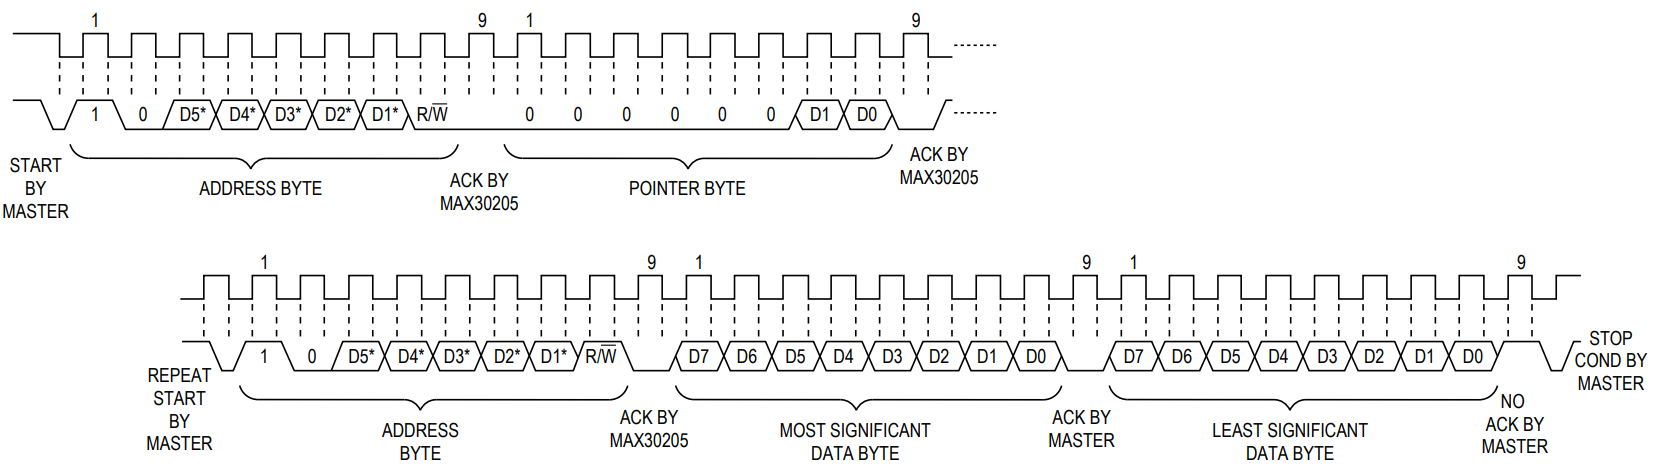
\includegraphics[width=1\textwidth]{AvancesPruebas/imagenes/diagramaI2C.png}}
	\caption{Diagrama de tiempo MAX30205.}
	\label{fig:DiagramaMAX30205}
\end{figure}

El procedimiento que se llevó a cabo para cumplir con los pasos establecidos en el diagrama de tiempo del sensor se describe a continuación.

\begin{enumerate}
	\item Se generó una condición de ''start'' para el bus I2C y de esa forma comenzar la comunicación entre ambos componentes.
	\item Antes de comenzar la lectura de información, el maestro debe conocer la dirección del esclavo, para esto
	\item  
\end{enumerate}


%El microcontrolador fue configurado como maestro y el sensor como esclavo, por lo que el maestro debe iniciar la comunicación, recibir los datos del sensor y terminar la comunicación.\\

%El código y descripción de las rutinas creadas para las operaciones anteriores se muestra a continuación.\\
%
%
%Rutina que genera la condición de \textbf{start} al bus I2C.
%{\small
%\begin{lstlisting}[frame=single]
%_START_I2C:
%	BCLR	IFS0,	#MI2CIF
%	BSET	I2CCON,	#SEN
%ESPERA_START:
%	BTSS	IFS0,	#MI2CIF
%	GOTO	ESPERA_START
%RETURN
%\end{lstlisting}
%}
%
%
%Esta rutina manda un dato de 8 bits al sensor de temperatura que es el dispositivo esclavo.	
%{\small
%\begin{lstlisting}[frame=single]
%
%ENVIA_DATO_I2C:
%	BCLR	IFS0,	#MI2CIF
%	
%	MOV.B	WREG,	I2CTRN
%ESPERA_ENVIA_DATO_I2C:
%	BTSS	IFS0,	#MI2CIF
%	GOTO	ESPERA_ENVIA_DATO_I2C
%	RETURN
%\end{lstlisting}
%}
%
%Rutina que recibe un dato de 8 bits del dispositivo esclavo que es el sensor de temperatura.
%{\small
%\begin{lstlisting}[frame=single]
%_RECIBE_DATO_I2C:
%	BCLR	IFS0,	#MI2CIF
%	BSET	I2CCON,	#RCEN
%ESPERA_RECIBE_DATO_I2C:
%	BTSS	IFS0,	#MI2CIF
%	GOTO	ESPERA_RECIBE_DATO_I2C
%	MOV		I2CRCV,	W0	
%	RETURN
%\end{lstlisting}
%}
%
%Después de realizar el programa, se conectó el sensor de temperatura al microcontrolador a través de las terminales SCL y SDA del mikrobus2 como se muestra en las figuras \ref{fig:ConexionMAX30205} y \ref{fig:ConexionFisicaMAX30205}.\\
%
%\begin{figure}[htbp!]
%	\centering
%	\fbox{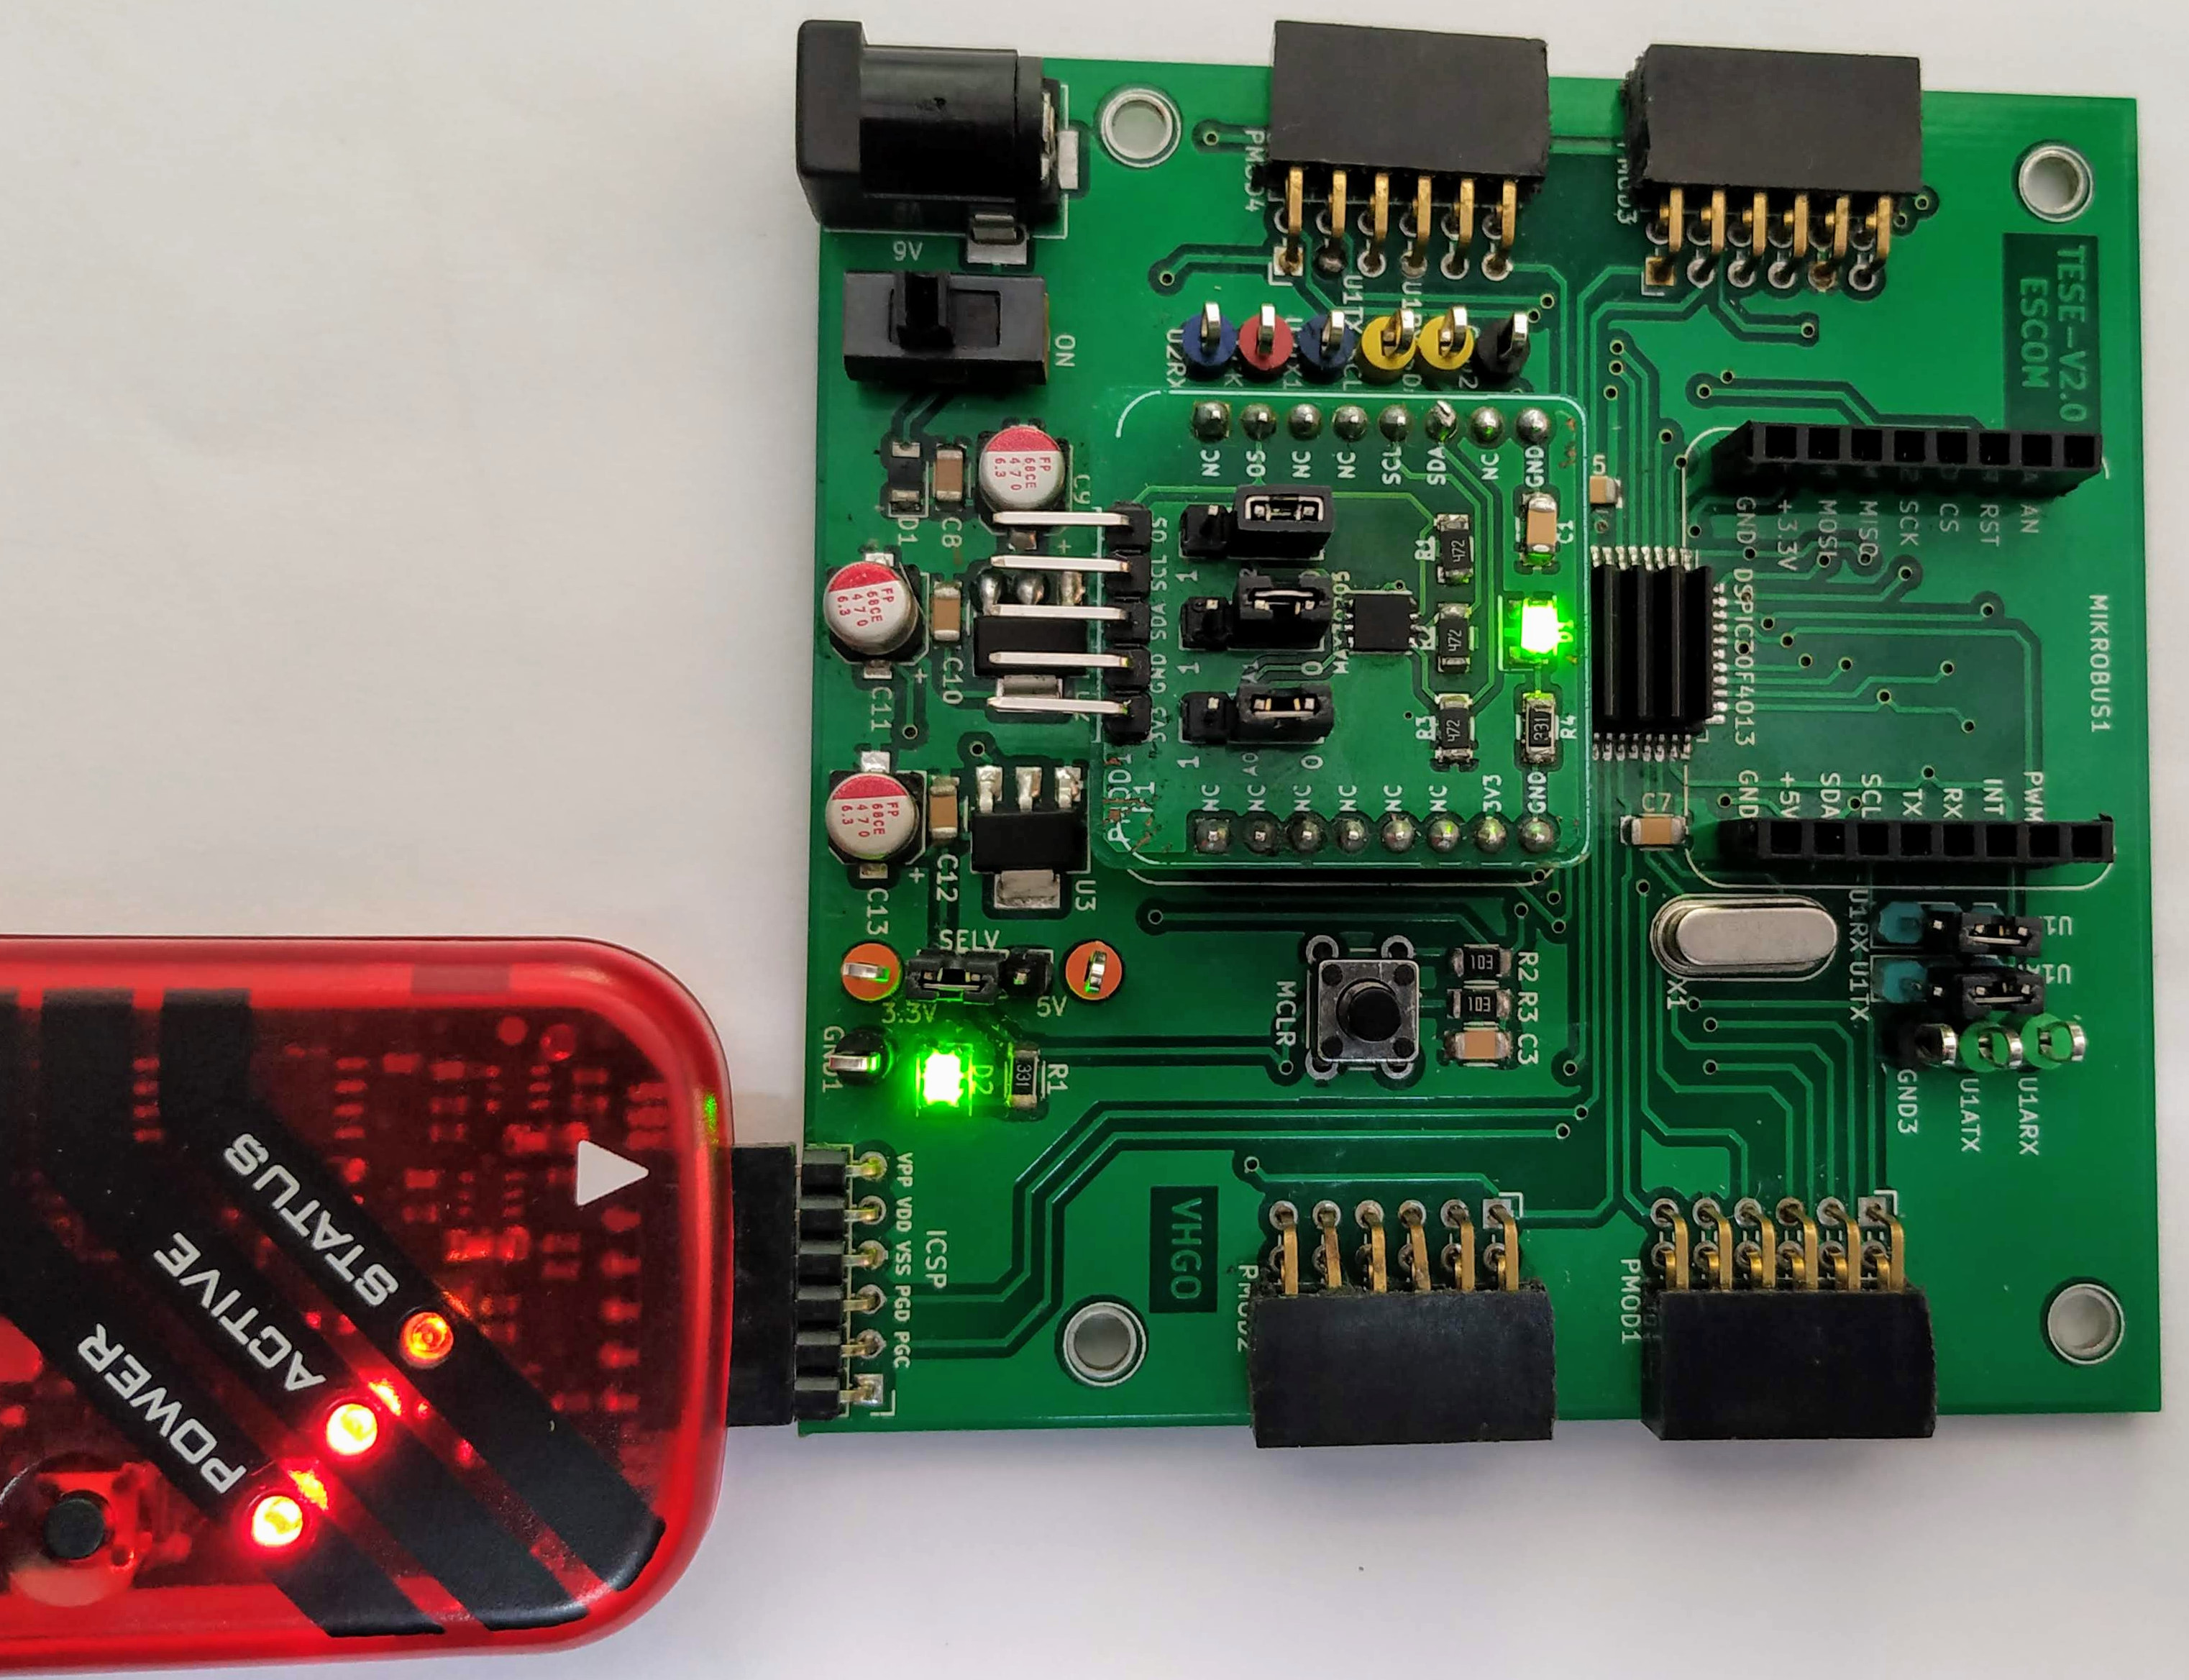
\includegraphics[width=0.8\textwidth]{AvancesPruebas/imagenes/MAX30205ConexionFisica.jpg}}
%	\caption{Conexión física del sensor MAX30205.}
%	\label{fig:ConexionFisicaMAX30205}
%\end{figure}
%
%\begin{figure}[htbp!]
%	\centering
%	\fbox{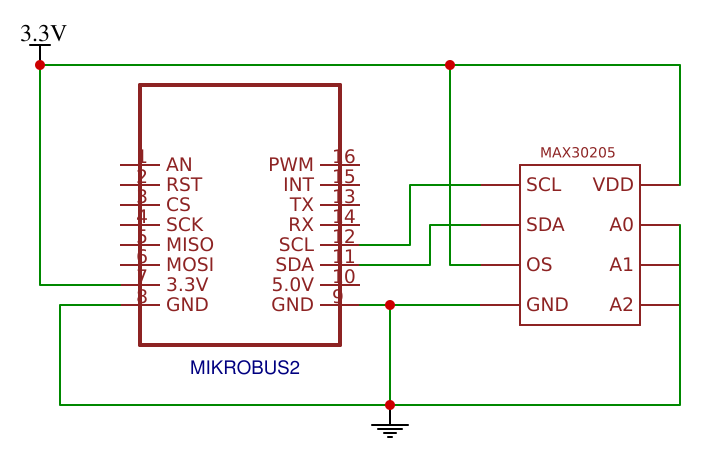
\includegraphics[width=0.7\textwidth]{AvancesPruebas/imagenes/MAX30205Conexion.png}}
%	\caption{Conexión del sensor MAX30205.}
%	\label{fig:ConexionMAX30205}
%\end{figure}

Para visualizar los datos recibidos del sensor, se habilitaron las terminales del UART1 y se conectó el módulo FT232 a la computadora. El resultado de la ejecución del programa con las mediciones leídas se muestra en la figura \ref{fig:ResultadoTerminalMAX30205}.\\


\begin{figure}[htbp!]
	\centering
	\fbox{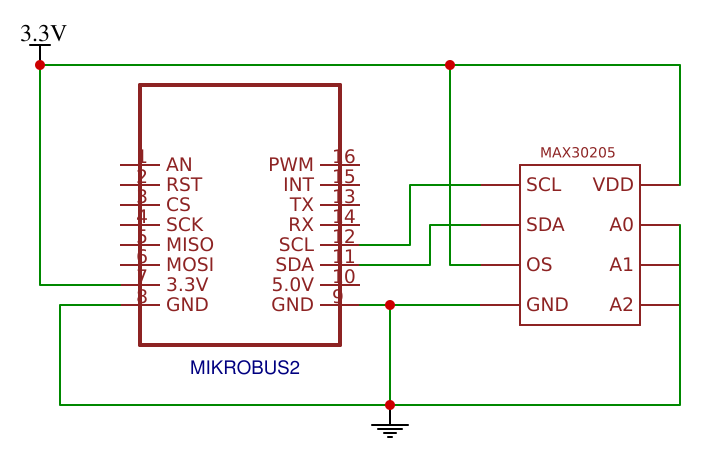
\includegraphics[width=0.7\textwidth]{AvancesPruebas/imagenes/MAX30205Conexion.png}}
	\caption{Conexión del sensor MAX30205.}
	\label{fig:ResultadoTerminalMAX30205}
\end{figure}

El resultado de esta prueba muestra que el sensor de temperatura MAX30205 funciona de manera esperada y la elección realizada fue correcta.

\clearpage